\documentclass[border=3pt]{standalone}
\usepackage{xcolor}
\usepackage{tikz}
\usetikzlibrary{arrows.meta,decorations.pathreplacing,positioning}

\definecolor{routeblue}{HTML}{2563EB}
\definecolor{routeorange}{HTML}{EA580C}
\definecolor{routeink}{HTML}{1E293B}

\begin{document}
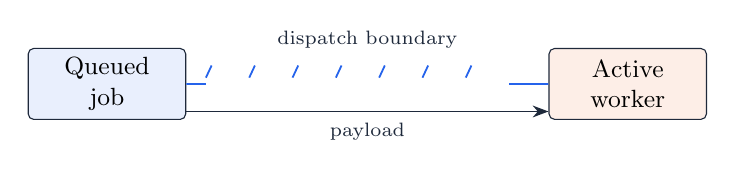
\begin{tikzpicture}[
  >=Stealth,
  stage/.style={draw=routeink,rounded corners=2pt,minimum width=2cm,
    minimum height=.9cm,align=center,font=\small},
  note/.style={font=\scriptsize,fill=white,inner sep=1.2pt,text=routeink}
]
  \node[stage,fill=routeblue!10] (queue) {Queued\\job};
  \node[stage,fill=routeorange!10,right=4.6cm of queue] (worker) {Active\\worker};

  \draw[routeblue,line width=.65pt,decorate,
    decoration={border,segment length=5.5mm,amplitude=1.7mm,angle=65,
      pre length=2.5mm,post length=4mm,raise=.8mm}]
    (queue.east) -- node[note,above=4mm] {dispatch boundary} (worker.west);
  \draw[-Stealth,routeink,line width=.6pt]
    ([yshift=-3.5mm]queue.east) -- node[note,below=1mm] {payload}
    ([yshift=-3.5mm]worker.west);
\end{tikzpicture}
\end{document}
